\chapter{General Kernel Spectral Method}
\label{chap:general-kernel-spectral-method}

\begin{figure}[H]
  \centering
  \label{fig:morse-operator}
  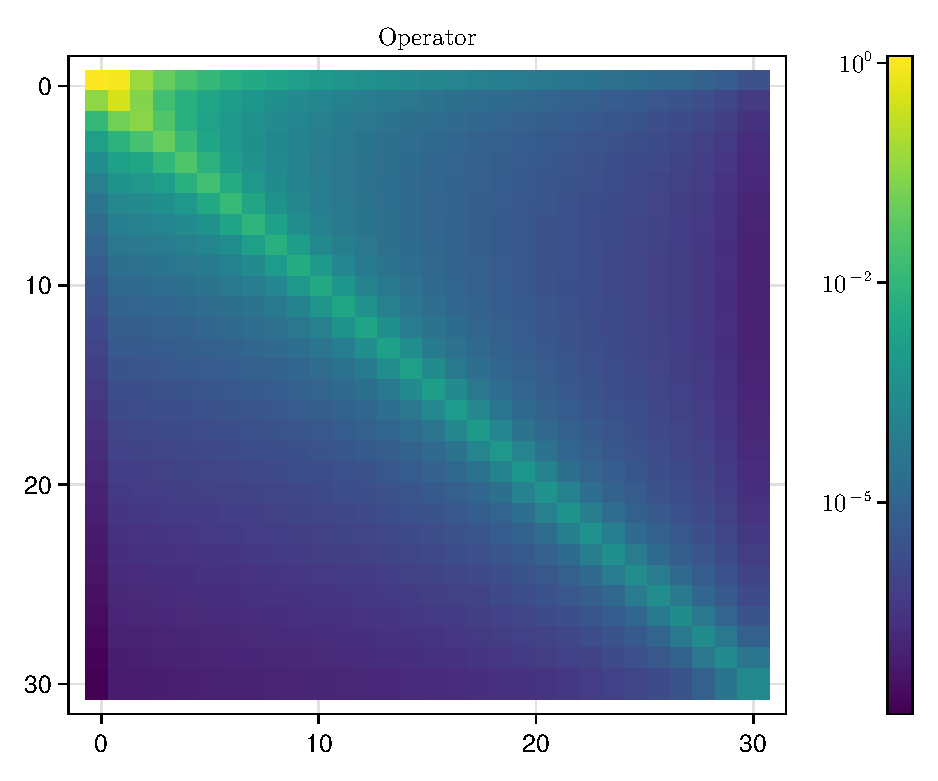
\includegraphics[width=0.5\linewidth]{results/morse/full-operator.pdf}
  \caption[]{Operator}
\end{figure}

\begin{figure}[H]
  \centering
  \label{fig:morse-solution-increasing-order}
  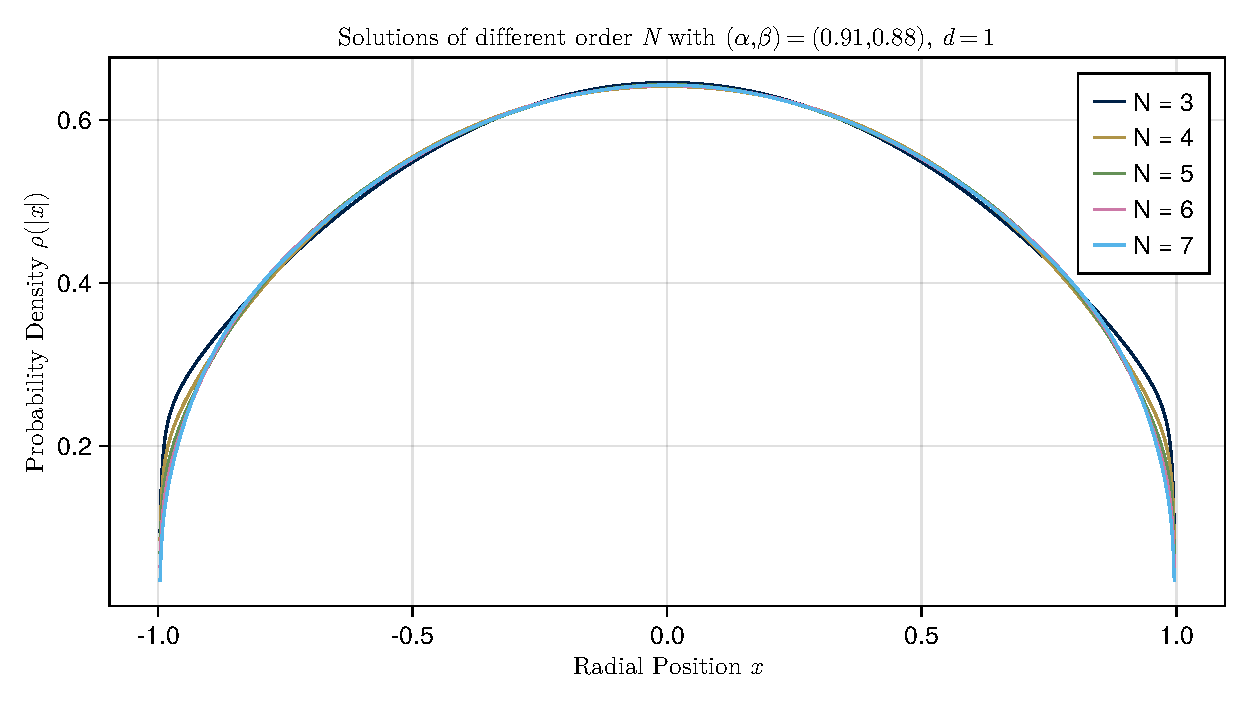
\includegraphics[width=0.8\linewidth]{results/morse/solution-increasing-order.pdf}
  \caption[]{Solutions of increasing orders}
\end{figure}

\begin{figure}[H]
  \centering
  \label{fig:monomial-solutions}
  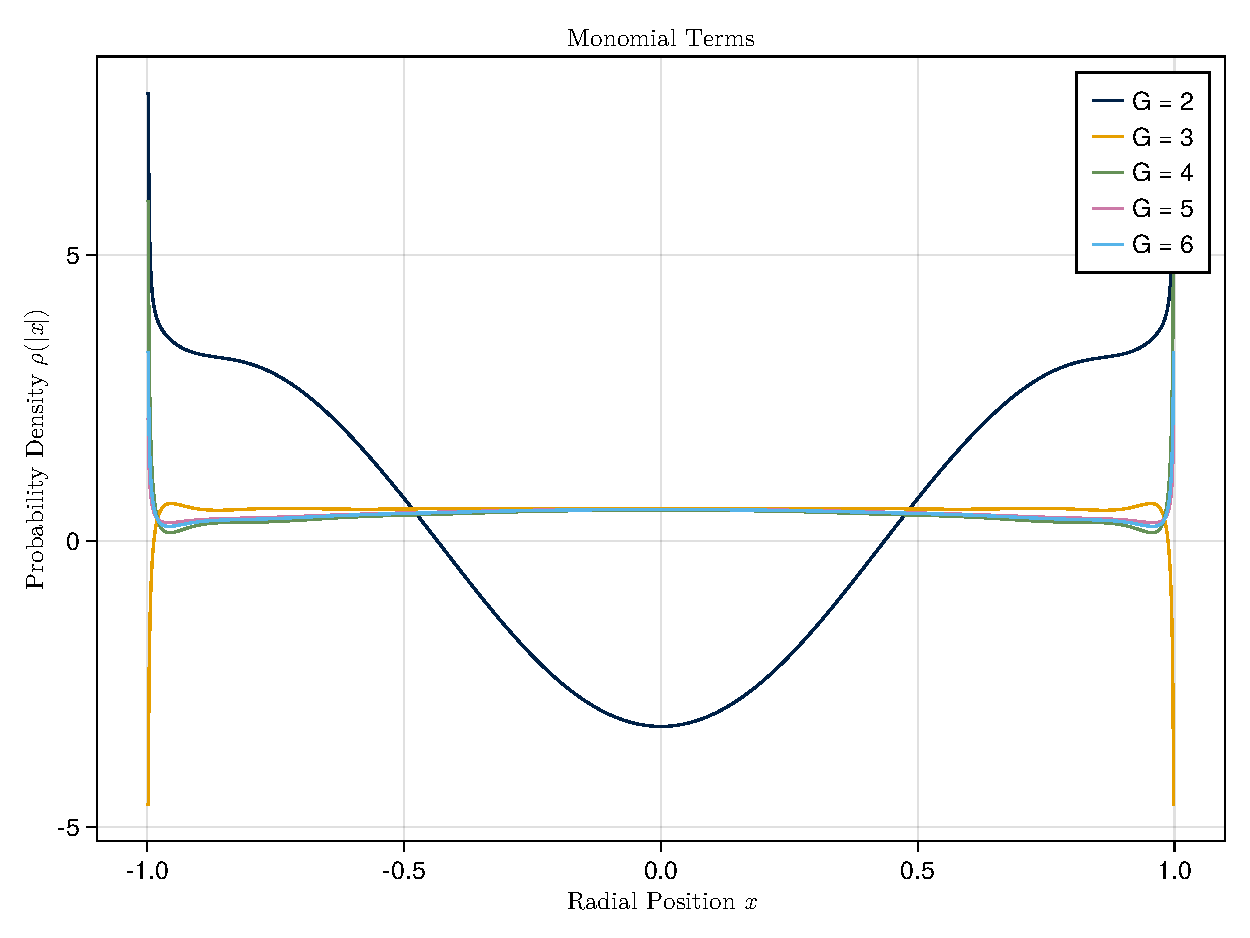
\includegraphics[width=0.7\linewidth]{results/morse/monomial-solutions.pdf}
  \caption[]{Solution for an increasing number of terms in the monomial expansion of the general kernel.}
\end{figure}

\begin{figure}[H]
  \centering
  \label{fig:monomial-basis-convergence}
  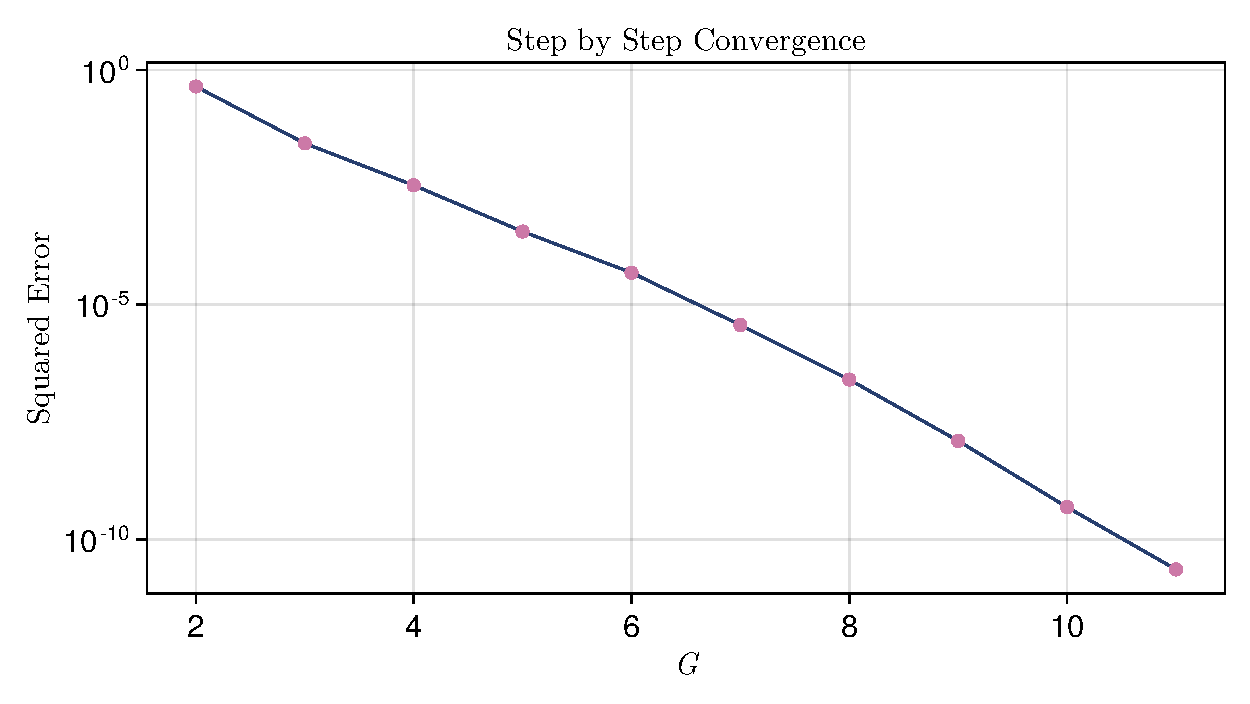
\includegraphics[width=0.7\linewidth]{results/morse/monomial-basis-convergence.pdf}
  \caption[]{Convergence}
\end{figure}

\begin{figure}[H]
  \centering
  \label{fig:varying-R-solutions}
  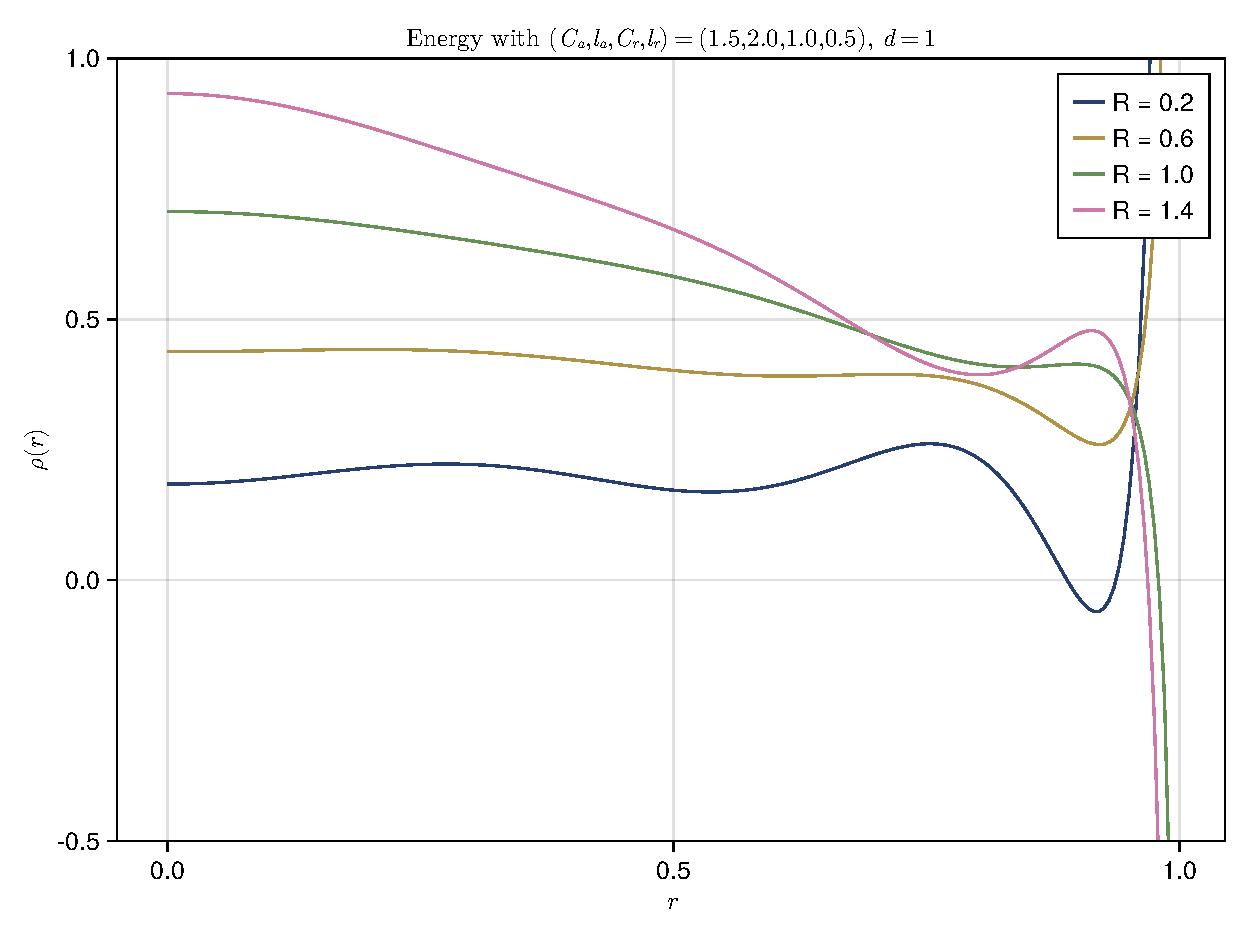
\includegraphics[width=0.7\linewidth]{results/morse/varying-R-solutions.pdf}
  \caption[]{Solutions with varying $R$.}
\end{figure}
